\section{Технический проект}

\subsection{Общая характеристика решения задачи}

Задача дипломного проекта заключается в разработке программного аудиопроцессора — универсального программного комплекса для обработки аудиосигналов в реальном времени на персональном компьютере. Процессор реализует цепочку современных аудиоэффектов с возможностью гибкой настройки, а также поддерживает многополосную обработку сигнала, что позволяет применять различные параметры эффектов к разным частотным диапазонам.

Разработка аудиопроцессора, способного выполнять обработку аудиосигнала с применением эквализации, многополосной компрессии, реверберации и шумоподавления.

Входные данные:
\begin{itemize}
	\item аудиосигнал в виде цифрового потока; 
	\item настройки эффектов, задаваемые пользователем (параметры эквалайзера, компрессора, реверберации и шумоподавления).
\end{itemize}

Выходные данные:
\begin{itemize}
	\item обработанный аудиосигнал, выводимый на устройство воспроизведения или сохраняемый в файл; 
	\item возможность мониторинга и визуализации параметров обработки в виде отображения формы волны или АЧХ.
\end{itemize}

\subsection{Обоснования выбора технологии проектирования}

На сегодняшний день рынок программных решений для обработки аудиосигналов активно развивается и предлагает множество продуктов, позволяющих достигать высокого качества звука в различных сферах — от профессиональной звукозаписи до бытового использования. Рост спроса на качественную цифровую обработку звука обусловлен увеличением популярности потоковых сервисов, подкастов, онлайн-трансляций и домашних студий, что делает актуальной задачу создания универсального и гибкого аудиопроцессора с возможностью многополосной обработки и применения современных эффектов.

Разработка собственного программного аудиопроцессора позволяет получить инструмент, адаптированный под конкретные требования пользователя, с возможностью расширения и оптимизации производительности. Такой подход отвечает современным тенденциям рынка, где востребованы решения с низкой задержкой, высокой точностью обработки и удобным управлением параметрами, что особенно важно в условиях реального времени.

Таким образом, выбранный подход к проектированию кода обусловлен необходимостью создания эффективного, масштабируемого и современного аудиопроцессора, который может конкурировать с существующими решениями и удовлетворять растущие потребности пользователей в качественной обработке звука.

\subsubsection{ Описание используемых технологий и языков программирования}

Для разработки аудиопроцессора был выбран язык программирования Python, что обусловлено рядом ключевых факторов:
\begin{enumerate}
	\item Простота и читаемость кода. Синтаксис Python близок к псевдокоду, что облегчает понимание и сопровождение проекта, а также позволяет быстро экспериментировать с алгоритмами обработки звука.
	\item Широкий набор библиотек для цифровой обработки сигналов. Python обладает мощными библиотеками (NumPy, SciPy, pydub и др.), которые предоставляют готовые инструменты для работы с аудиоданными, фильтрами, преобразованиями и другими DSP-операциями. Это значительно ускоряет разработку и повышает надежность кода.
	\item Возможность оптимизации производительности. Для повышения скорости вычислений в критичных местах применяется JIT-компиляция с помощью Numba, что позволяет добиться близкой к нативной производительности без перехода на более низкоуровневые языки.
	\item Поддержка многопоточности и асинхронной обработки. В проекте используется ThreadPoolExecutor и другие средства стандартной библиотеки для параллельной обработки аудиоданных, что улучшает отзывчивость и снижает задержки при работе в реальном времени.
	\item Гибкость и расширяемость архитектуры. Модульный подход с использованием классов и четким разделением функционала (например, отдельные классы для компрессоров, эквалайзеров и ревербераторов) позволяет легко добавлять новые эффекты и модифицировать существующие.
	\item Активное сообщество и наличие обучающих материалов. Благодаря большому количеству статей, учебников и примеров по цифровой обработке сигналов на Python, разработка и отладка проекта становится более эффективной.
\end{enumerate}

Таким образом, выбор Python и сопутствующих технологий проектирования обусловлен их оптимальным сочетанием простоты, функциональности и производительности, что отвечает требованиям дипломного проекта по созданию программного аудиопроцессора с возможностью обработки в реальном времени и расширяемой архитектурой.

\subsubsection{Язык программирования Python}

Python — это высокоуровневый, интерпретируемый язык программирования общего назначения, который отличается простотой, универсальностью и мощной функциональностью. Он был разработан в конце 1980-х годов Гвидо ван Россумом с целью создания языка с понятным и читаемым синтаксисом, что делает его идеальным как для начинающих программистов, так и для профессионалов. В Python используется динамическая строгая типизация, а весь код выполняется интерпретатором, что позволяет быстро находить и исправлять ошибки во время разработки. Особенностью языка является выделение блоков кода с помощью отступов, что повышает читаемость и структурированность программ. Python поддерживает множество парадигм программирования, включая объектно-ориентированное, процедурное, функциональное и асинхронное программирование, а также метапрограммирование, что делает его гибким и мощным инструментом для решения самых разных задач.

Преимущества Python:
\begin{itemize}
	\item легкость изучения и быстрота написания кода;
	\item высокая читаемость и поддерживаемость программ;
	\item универсальность и широкая сфера применения;
	\item возможность быстрой прототипизации и разработки сложных систем;
	\item поддержка современных парадигм программирования.
\end{itemize}

Недостатки Python:
\begin{itemize}
	\item относительно низкая скорость выполнения по сравнению с компилируемыми языками;
	\item ограничения многопоточности из-за глобальной блокировки интерпретатора (GIL);
	\item не всегда подходит для задач низкоуровневого программирования и высокопроизводительных приложений.
\end{itemize}

Python является одним из самых популярных языков программирования благодаря своему балансу простоты, гибкости и мощи, что делает его оптимальным выбором для широкого спектра проектов — от обучения и научных исследований до промышленной разработки и создания сложных программно-информационных систем.

В коде используются следующие библиотеки Python:
\begin{itemize}
	\item NumPy - обеспечивает высокопроизводительные вычисления с многомерными массивами, что критично для обработки аудиоданных, представленных в виде временных рядов;
	\item SciPy - используется для реализации цифровых фильтров (эквалайзер), БПФ (анализ спектра) и других математических операций;
	\item PyDub - библиотека для работы с аудиофайлами, предоставляющая: простые методы загрузки и сохранения в форматах WAV, MP3, OGG, FLAC, базовые операции, такие как обрезка, наложение, изменение громкости, конвертация частоты дискретизации, интеграцию с FFmpeg для поддержки дополнительных кодеков;
	\item Soundfile используется для чтения и записи аудиофайлов различных форматов, обеспечивая удобный доступ к аудиоданным на диске, позволяет загружать исходные аудиозаписи и сохранять результаты обработки без потери качества;
	\item SoundDevice - обеспечивает низкоуровневый доступ к аудиоустройствам через PortAudio. Ключевые функции: воспроизведение и запись в реальном времени с минимальной задержкой, поддержка ASIO, WASAPI, Core Audio для профессиональных аудиоинтерфейсов, гибкая настройка параметров потока: частота дискретизации, размер буфера, количество каналов;
	\item Matplotlib - используется для визуализации аудиоданных: построение осциллограмм (форма сигнала во временной области), отображение АЧХ (амплитудно-частотных характеристик) с логарифмической шкалой, интерактивное обновление графиков в реальном времени;
	\item Threading и concurrent.futures — стандартные библиотеки Python для организации многопоточной и параллельной обработки;
	\item Tkinter - стандартная библиотека Python для создания графического интерфейса. В проекте применяется для: построения основного окна с вкладками (эквалайзер, компрессор, реверберация), реализации интерактивных элементов: ползунки, кнопки, метки, интеграции графиков Matplotlib через FigureCanvasTkAgg;
	\item Numba - JIT-компилятор для оптимизации вычислительно сложных участков кода: ускорение алгоритмов компрессии и реверберации в 5–10 раз, поддержка многопоточности.
\end{itemize}

\subsubsection{Кроссплатформенная библиотека FFmpeg}

FFmpeg — это мощная кроссплатформенная библиотека для обработки мультимедиа, используемая в проекте для работы с аудиофайлами различных форматов. Взаимодействие с FFmpeg осуществляется через обёртку PyDub, что значительно упрощает операции чтения, записи и конвертации аудио.

Основные функции FFmpeg в проекте:
\begin{enumerate}
	\item Поддержка множества аудиоформатов. Позволяет загружать и сохранять файлы в форматах: без сжатия: WAV, AIFF, с потерями: MP3, AAC, OGG, без потерь: FLAC, ALAC. Обеспечивает автоматическое определение кодека при загрузке.
	\item Конвертация аудио: изменение частоты дискретизации, преобразование между форматами, конвертация числа каналов.
	\item Нормализация и обработка. Автоматическая регулировка громкости.
\end{enumerate}

FFmpeg был выбран по рядам преимуществ:
\begin{itemize}
	\item универсальность: поддержка 100+ кодеков и контейнеров;
	\item стабильность: отлаженные алгоритмы декодирования/кодирования;
	\item производительность: оптимизированные нативные библиотеки;
	\item гибкость: Возможность тонкой настройки параметров через командные опции.
\end{itemize}

\subsection{Эффекты}

\subsubsection{Устройство эквалайзера}

Эквалайзер — это устройство или программный алгоритм, предназначенный для корректировки амплитудно-частотной характеристики (АЧХ) звукового сигнала. Он позволяет усиливать или ослаблять определённые частотные диапазоны, изменяя тембр звука. Эквалайзер работает, разделяя входной аудиосигнал на несколько частотных полос (диапазонов), каждая из которых обрабатывается отдельно. После обработки всех полос сигналы складываются, и на выходе получается звук с изменённой частотной характеристикой.

В программе реализован цифровой параметрический эквалайзер, у которого есть три полосы частот, а так же коррекция их по громкости в децибелах. Такие эквалайзеры часто используются в профессиональной звукозаписи и сведении аудио.

Цифровой IIR-фильтр (Биквадратный, на основе Баттерворта)

IIR-фильтр (Infinite Impulse Response — бесконечная импульсная характеристика) — это тип цифрового фильтра, который использует обратную связь, благодаря чему может иметь очень крутые склоны АЧХ при малом порядке.

Биквадратный фильтр (Biquad) — это частный случай IIR-фильтра 2-го порядка, который реализуется с помощью разностного уравнения и часто используется в эквалайзерах из-за своей эффективности.

Фильтр Баттерворта — один из самых популярных типов фильтров, обеспечивающий максимально гладкую АЧХ в полосе пропускания без пульсаций.

Этот эквалайзер обеспечивает:
\begin{itemize}
	\item низкую задержку (важно для реального времени);
	\item минимальные фазовые искажения;
	\item точную обработку частот;
	\item защиту от перегрузки.
\end{itemize}

\subsubsection{Устройство многополосного компрессора}

Многополосный компрессор — устройство динамической обработки аудиосигнала, предназначенное для управления динамическим диапазоном звука с разделением сигнала на несколько частотных полос. Основная идея многополосного компрессора заключается в том, что входящий аудиосигнал сначала разделяется на несколько частотных диапазонов с помощью цифровых фильтров, после чего каждая полоса обрабатывается отдельным компрессором с индивидуальными параметрами. Такой подход позволяет более точно и эффективно контролировать динамику звука в каждом частотном диапазоне, сохраняя при этом естественность звучания и минимизируя искажения.

В реализованном компрессоре разделение сигнала осуществляется с использованием цифровых фильтров, которые выделяют низкочастотную, среднечастотную и высокочастотную полосы. Для каждой полосы создаётся отдельный компрессорный блок, реализованный в виде программного модуля, который обрабатывает сигнал независимо от других полос. Каждый из этих блоков имеет собственные настройки ключевых параметров компрессии:
\begin{itemize}
	\item Threshold (порог);
	\item Ratio (коэффициент компрессии); 
	\item Attack (атака);
	\item Release (восстановление);
	\item Knee (характеристика перехода);
	\item Make-up Gain (компенсационное усиление).
\end{itemize}

Порог срабатывания определяет уровень громкости, при превышении которого начинается сжатие сигнала. Коэффициент сжатия задаёт степень уменьшения динамического диапазона, то есть насколько сильно будет снижаться громкость сигналов, превышающих порог. Время атаки регулирует скорость срабатывания компрессора после превышения порога, а время релиза — скорость возврата усиления к исходному уровню после снижения входного сигнала ниже порога, характеристика перехода определяет плавный переход от отсутствия сжатия к активному сжатию сигнала, компенсационное усиление позволяет регулировать сигнал после обработки, чтобы вернуть ему исходную громкость. Эти параметры позволяют гибко настраивать реакцию компрессора на изменения громкости в каждой полосе, обеспечивая плавное и естественное звучание.

В основе алгоритма компрессии лежит вычисление коэффициента усиления (gain reduction), который применяется к аудиосигналу полосы. Этот коэффициент рассчитывается на основе текущего уровня сигнала и параметров компрессии с учётом сглаживания изменения усиления для предотвращения резких артефактов в звуке. Для повышения производительности вычисления оптимизированы с помощью JIT-компиляции (Numba), а обработка полос может выполняться параллельно с использованием многопоточности, что обеспечивает минимальную задержку и возможность работы в реальном времени.

Таким образом, многополосный компрессор, реализованный в проекте, представляет собой совокупность нескольких параллельных компрессоров, каждый из которых отвечает за свой частотный диапазон и имеет независимые настройки. Это обеспечивает высокую гибкость и качество динамической обработки, позволяя адаптировать параметры под особенности конкретного аудиоматериала и задачи. Использование цифровых фильтров для разделения сигнала и оптимизированных алгоритмов компрессии обеспечивает эффективную работу устройства в реальном времени, что соответствует современным требованиям к аудиопроцессорам.

\subsubsection{Устройство реверберации}

FDN (Feedback Delay Network) — это один из самых мощных алгоритмов цифровой реверберации, используемый для создания реалистичных пространственных эффектов. Он основан на множестве линий задержки с обратной связью, образующих сложную сеть, имитирующую отражения в помещении.

Принцип работы:
\begin{itemize}
	\item входной сигнал разделяется на несколько параллельных линий задержки, каждая из которой задерживает сигнал на разное время;
	\item после задержки сигнал проходит через фильтр демпфирования (имитация потери высоких частот);
	\item затем он умножается на коэффициенты матрицы обратной связи, определяющей, какая часть сигнала возвращается в каждую линию;
	\item обновлённый сигнал снова поступает на вход линий задержки;
	\item результирующий реверберационный сигнал формируется как сумма выходов всех линий.
\end{itemize}

Ключевые особенности FDN:
\begin{itemize}
	\item реалистичность — лучше имитирует поздние отражения, чем алгоритмы на основе простых задержек;
	\item гибкость — можно настраивать время реверберации, демпфирование и пространственность;
	\item стабильность — ортогональная матрица гарантирует отсутствие бесконечного нарастания.
\end{itemize}

\subsection{Архитектура программно-информационной системы}

На рисунке \ref{DiagramArch:image} представлена многослойная архитектура системы с чётким разделение ответственности между компонентами.

\begin{figure}[p]  % Разместить на отдельной странице
	\centering
	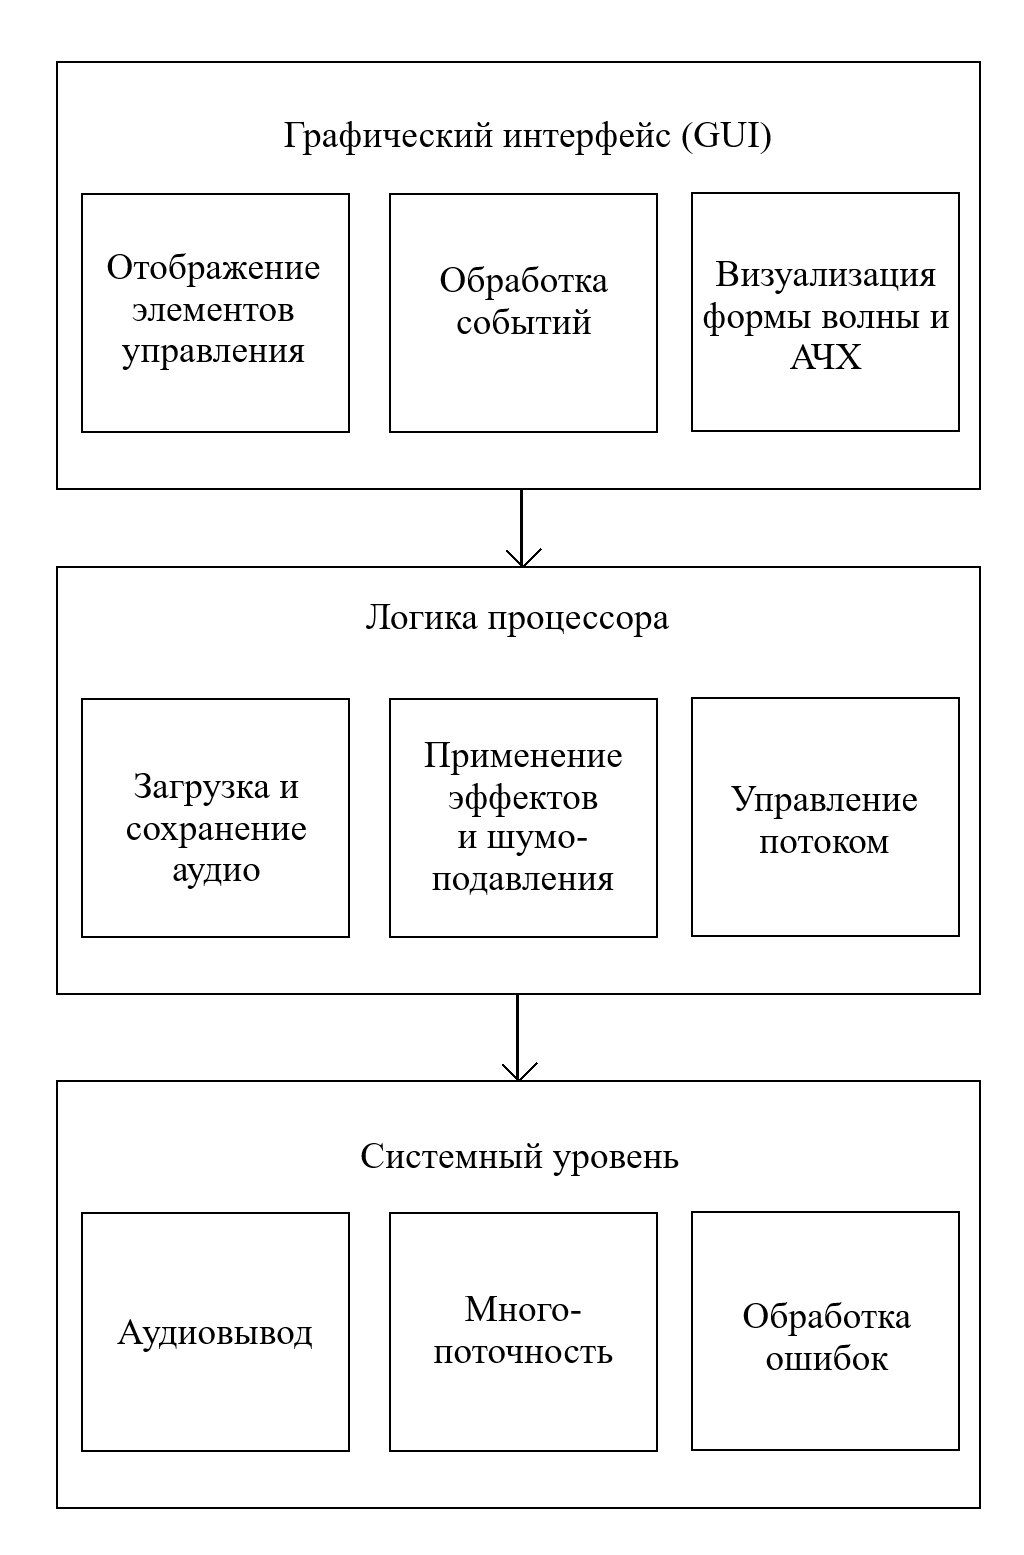
\includegraphics[width=0.8\linewidth]{DiagramArch}
	\caption{Архитектура программно-информационной системы}
	\label{DiagramArch:image}
\end{figure}
\clearpage

\begin{enumerate}
	\item Графический интерфейс отображает элементы управления (кнопки, ползунки, вкладки), визуализирует аудиоданные в реальном времени (Форма волны, АЧХ), обрабатывает пользовательские события (нажатия кнопок, изменение параметров).
	\item Логика процессора отвечает за загрузку/сохранение аудио, чтение файлов через PyDub/FFmpeg, конвертирует в формат float32 для обработки. Применяет эффекты: шумоподавление, эквалайзер (БИХ-фильтры для 8 полос регулировки частот), многополосный компрессор (динамическое сжатие с параметрами), реверберация. Буферизирует данные и синхронизирует позицию воспроизведения.
	\item На уровне системы происходит ввод и вывод аудио, создаётся отдельный поток для обработки аудио и очереди для передачи данных между потоками. Обрабатываются ошибки, перехватываются исключения и логируются в файл.
\end{enumerate}

\begin{itemize}
	\item графический интерфейс включает главное окно, состоящее из кнопок управление воспроизведением и загрузки/сохранения, вкладок эффектов (эквалайзер, компрессор и ревербератор), окна отображение визуализации формы волны и АЧХ;
	\item логика процессора читает и обрабатывает аудиофайлы, применяется выбранные эффекты по очереди, управляет всей работой программы;
	\item системное устройство воспроизводит звук, работает с файлами, открывает и сохраняет их, управляет несколькими задачами одновременно;
	\item вспомогательные модули включают частотный анализ, автоматически регулирует громкость и записывает ошибки и события.
\end{itemize}

Все части программы взаимодействуют между собой по чётким правилам. Когда пользователь меняет настройки, интерфейс передаёт их в модуль обработки, который применяет эффекты и отправляет результат на воспроизведение и отображение. Для плавной работы использовались очереди задач для работы в многопоточном режиме, оптимизирует сложные вычисления для быстрой работы.

\subsection{Архитектура приложения}

Приложение построено по многослойной модульной архитектуре с разделением на логические компоненты, взаимодействующие через четко определенные интерфейсы. В основе лежит ядро обработки аудиосигналов, окруженное графическим интерфейсом, системными сервисами и вспомогательными модулями.
Графический интерфейс реализован на Tkinter и включает:
\begin{itemize}
	\item главное окно (MainWindow) с вкладками для управления эффектами, кнопками воспроизведения/паузы и областью визуализации;
	\item панель эквалайзера (EQPanel) с восьмью ползунками, отображающая АЧХ через Matplotlib;
	\item панель компрессора (CompressorPanel) для настройки порога, сжатия, атаки, восстановления, характеристики перехода, усиления;
	\item панель реверберации (ReverbPanel) для настройки эффект, сухой сигнал, размер комнаты, затухание;
	\item визуализатор спектра (SpectrumAnalyzer), отображающий осциллограмму (форма сигнала) и частотный спектр (БПФ) в реальном времени;
	\item прогресс-бар с управлением позицией воспроизведения и отображением длительности трека.	
\end{itemize}

Логический процессор — центральный модуль, отвечающий за:
\begin{itemize}
	\item загрузку и конвертацию аудио через PyDub (с использованием FFmpeg как бэкенда), включая поддержку WAV, MP3, FLAC;
	\item эквалайзер на БИХ-фильтрах с частотами 50 Гц, 150 Гц, 250 Гц, 500 Гц, 1 кГц, 3 кГц, 7 кГц, 15 кГц;
	\item компрессор с разделением на три диапазона частот, в каждом из которых есть регулировки: treshold, ratio, knee, attack, rrelease, gain;
	\item реверберация на основе алгоритма Schroeder (комбинация линий задержки и FIR-фильтров);
	\item буферизацию данных для плавного воспроизведения и нормализацию уровня сигнала.
\end{itemize}

Системный слой обеспечивает интеграцию с ОС и оборудованием:
\begin{itemize}
	\item аудиопоток (AudioStream) на базе SoundDevice, обрабатывающий ввод/вывод в реальном времени с настройкой latency и sample rate (44.1–192 кГц);
	\item менеджер потоков (ThreadManager) для параллельной обработки (отдельные потоки для: GUI, аудиообработки, визуализации);
	\item файловый менеджер (FileManager) с кэшированием загруженных треков и поддержкой метаданных (ID3-теги).
\end{itemize}

Архитектура обеспечивает масштабируемость (добавление новых эффектов через модули), производительность (JIT-компиляция, многопоточность) и отказоустойчивость (изоляция сбоев в отдельных потоках).

\subsection{Проект данных программно-информационной системы}

Система оперирует тремя основными категориями данных: входными, промежуточными и выходными. Входные данные включают аудиофайлы в форматах WAV, MP3, FLAC и OGG с поддержкой различных характеристик (битность 16-24 бит, частота дискретизации 44.1-192 кГц), а также параметры эффектов, настраиваемые пользователем через графический интерфейс. Для эквалайзера это уровни усиления по восьми полосам (50 Гц, 150 Гц, 250 Гц, 500 Гц, 1 кГц, 3 кГц, 7 кГц, 15 кГц с диапазоном ±24 дБ), для каждого диапазона компрессора — порог срабатывания от -60 до 0 дБ, коэффициент компрессии от 1:1 до 10:1, характеристика перехода от 0 до 100, время атаки от 0.1 до 100 мс, время восстановления от 10 до 1000 мс, усиление от -20 до +20 дБ, для реверберации — соотношение обработанного и исходного сигнала, виртуальный размер помещения, затухание, две регулировки среза верхних и нижних частот, панорамирование.

Промежуточные данные представлены в виде нормализованных аудиобуферов в формате 32-битных чисел с плавающей запятой, организованных как моно- или стереоканальные массивы. Система использует кольцевые буферы для обработки в реальном времени и промежуточные спектральные данные, полученные через быстрое преобразование Фурье с применением оконной функции. Для хранения состояния эффектов используются специализированные структуры: коэффициенты БИХ-фильтров эквалайзера, параметры огибающей компрессора и линии задержки реверберации.

Выходные данные включают обработанные аудиофайлы в выбранных пользователем форматах (WAV с PCM-кодированием или MP3 с переменным битрейтом), сохраняющие исходные параметры частоты дискретизации или конвертируемые к стандартным значениям. Визуализационные данные содержат три основных компонента: осциллограмму последних обработанных сэмплов, частотный спектр с разрешением 8192 точек и амплитудно-частотную характеристику активных фильтров, отображаемую в логарифмическом масштабе от 20 Гц до 20 кГц.

Метаданные системы включают пользовательские пресеты эффектов, содержащие полный набор параметров обработки, историю операций для возможности отмены действий, а также технические лог-файлы с информацией о производительности и ошибках. Все данные передаются между компонентами системы через единый формат аудиоблоков, сопровождаемых метаинформацией о текущих настройках обработки, что обеспечивает согласованность работы многопоточной архитектуры.

\subsubsection{Описание сущностей графического интерфейса}

Графический интерфейс Audio Processor представляет собой комплекс взаимосвязанных визуальных компонентов, объединенных в единое интуитивное пространство. 

Интерфейс поддерживает несколько режимов отображения - компактный для мониторов с малым разрешением, расширенный с дополнительными инструментами анализа для профессиональной работы, и режим презентации с увеличенными элементами управления. Все визуальные компоненты реализованы с учетом эргономики - важные элементы выделены акцентным цветом, соблюдены принципы визуальной иерархии, обеспечена последовательная реакция на пользовательские действия. Особенностью интерфейса является синхронизация всех элементов - изменения параметров эффектов мгновенно отражаются на графиках, а действия пользователя сопровождаются тактильной обратной связью в виде тонких анимационных эффектов.

\subsubsection{Описание сущностей логики процессора}

Основу обработки составляет низкоуровневый модуль, работающий с потоком аудиосэмплов в формате 32-битных чисел с плавающей точкой, обеспечивающий базовые операции нормализации и передискретизации. Система эффектов построена вокруг трех ключевых процессоров: эквалайзер реализует трехполосную фильтрацию через каскад БИХ-фильтров с настраиваемыми частотами среза и коэффициентами усиления, компрессор отвечает за компрессию сигнала с алгоритмами расчета огибающей и адаптивными параметрами атаки/восстановления, а ревербератор генерирует реверберацию через комбинацию линий задержки с регулируемыми параметрами затухания.

Поток данных управляется специализированным менеджером маршрутизации, который обеспечивает передачу аудиоблоков между модулями с минимальной задержкой, используя кольцевые буферы и механизм синхронизации для многопоточной работы. Состояние системы отслеживает активные эффекты, параметры обработки и текущий режим работы (реальное время/оффлайн обработка), предоставляя единый интерфейс для управления конвейером обработки. 

\subsubsection{Описание сущностей системного уровня}

Системная архитектура приложения построена на нескольких ключевых компонентах, обеспечивающих интеграцию с операционной средой и аппаратными ресурсами. Центральным элементом выступает абстрактный слой взаимодействия с аудиодрайверами, реализующий поддержку ASIO, WASAPI и Core Audio через единый кроссплатформенный API. Для управления устройствами ввода-вывода используется DeviceManager, который автоматически обнаруживает доступные аудиоинтерфейсы, анализирует их характеристики и предоставляет унифицированный интерфейс для работы с ними.

Файловая подсистема основана на компоненте, объединяющем возможности стандартных Python-библиотек для работы с файлами и мощь FFmpeg для обработки мультимедиа. Этот модуль включает кэширующий механизм для ускорения повторного доступа к аудиофайлам и систему контроля целостности данных. 

Многопоточная архитектура координируется центральным диспетчером задач, который создает и управляет тремя основными типами потоков: высокоприоритетным аудиопотоком реального времени, фоновыми рабочими потоками для обработки эффектов и служебными потоками для визуализации и логирования.

\subsection{Проектирования пользовательского интерфейса}

Центральное место занимает динамическая визуализация аудиопотока - двойной дисплей с синхронизированными осциллограммой и АЧХ, выполненный в темной цветовой гамме с акцентными элементами салатового цвета для выделения ключевых параметров сигнала. Основная рабочая область: верхняя треть экрана отведена под графики, центральная часть содержит компактные панели эффектов с интуитивными регуляторами, а нижний сектор занимает расширенная панель транспорта с профессиональными элементами управления.

Навигационная система реализована через адаптивную панель вкладок с контекстно-зависимыми элементами управления - при выборе конкретного эффекта (эквалайзер, компрессор, реверберация) нижняя панель автоматически наполняется соответствующими регуляторами, сохраняя при этом быстрый доступ к основным функциям. Все элементы управления спроектированы с учетом тактильного взаимодействия - ползунки имеют выраженные рифленые ручки с магнитными точками для часто используемых значений, кнопки обладают трехступенчатой визуальной обратной связью (покой, наведение, нажатие), а переключатели сопровождаются мягкими анимационными переходами.

